
%
% -----
% The full Finite State Automata over inference states
% -----
%
\newcommand\completeFSA{
  \begin{tikzpicture}[shorten >=1pt,node distance=2.0cm,auto,semithick,inner sep=2pt,bend angle=15,
    % (styles)
    every state/.style={draw=red!50,very thick,fill=red!10},
    accepting/.style={draw=blue!50,very thick,fill=blue!10},
    initial/.style={draw=green!50,very thick,fill=green!10}
    ]

    % (states)
    \node[state,initial]   (equivalent)                             {\equivalent};
    \node[state,accepting] (reverse)    [above right=of equivalent] {\reverse};
    \node[state,accepting] (cover)      [right=of reverse]          {\cover};
    \node[state]           (negate)     [below right=of cover]      {\negate};
    \node[state,initial]   (forward)    [below right=of equivalent] {\forward};
    \node[state]           (alternate)  [right=of forward]          {\alternate};

    % (paths)
    \path[<->] (equivalent) edge              node {\negate}             (negate);
    \path[->]  (negate)     edge [bend right] node {\forward}            (cover)
                            edge [bend left]  node {\alternate}          (reverse)
                            edge [bend left]  node {\reverse}            (alternate)
                            edge [bend right] node {\cover}              (forward)
                            edge [loop right] node {\equivalent}         (negate)
               (reverse)    edge [bend left]  node {\negate\cover}       (cover)
                            edge [loop above] node {\reverse\equivalent} (reverse)
               (cover)      edge [bend left]  node {\negate\alternate}   (reverse)
                            edge [loop above] node {\forward\equivalent} (cover)
               (forward)    edge [bend left] node {\negate\alternate}   (alternate)
                            edge [loop below] node {\forward\equivalent} (forward)
               (alternate)  edge [bend left]  node {\negate\cover}       (forward)
                            edge [loop below] node {\reverse\equivalent} (alternate)
               ;
  \end{tikzpicture}
}

%
% -----
% A Finite State Automata for the collapsed inference states
% -----
%
\newcommand\collapsedFSA{
  \begin{tikzpicture}[shorten >=1pt,node distance=2.0cm,auto,semithick,inner sep=2pt,bend angle=30,
    % (styles)
    every state/.style={draw=red!50,very thick,fill=red!10},
    accepting/.style={draw=blue!50,very thick,fill=blue!10},
    initial/.style={draw=green!50,very thick,fill=green!10}
    ]

    % (states)
    \node[state,initial]   (valid)                               {$~~x \Rightarrow y~~$};
    \node[state,accepting] (unknown)    [above right=of valid]   {$~~x \nRightarrow y~~$};
    \node[state]           (invalid)    [below right=of unknown] {$x \Rightarrow \lnot y$};
    
    % (edges)
    \path[->]  (valid)      edge [bend left]  node {\negate\alternate}   (invalid)
                            edge [bend left]  node {\reverse\cover}      (unknown)
                            edge [loop left]  node {\equivalent\forward} (valid)
               (invalid)    edge [bend left]  node {\negate\cover}       (valid)
                            edge [bend right] node {\alternate\forward}  (unknown)
                            edge [loop right] node {\equivalent\reverse} (invalid)
               (unknown)    edge [loop above] node {any}                 (unknown)
               ;

  \end{tikzpicture}
}

%
% -----
% A Teaser Search Path
% -----
%
\newcommand\teaserSearch{
  \tikzstyle{level 1}=[level distance=1.5cm, sibling distance=3.5cm]
  \tikzstyle{level 2}=[level distance=1.5cm, sibling distance=2cm]
  \tikzstyle{level 3}=[level distance=1.5cm, sibling distance=2cm]
  \tikzstyle{level 4}=[level distance=1.5cm, sibling distance=2cm]
  \tikzstyle{fact} = [text width=7em, text centered]
  \tikzstyle{sink} = [text width=7em, text centered, 
                      rectangle, draw]
  \tikzset{
    goodPath/.style={draw=blue}
  }

  % "No carnivores eat animals"
  % false because: "The cat ate a mouse"

  \begin{tikzpicture}[grow=down, sloped]
  \node[fact] {\w{No carnivores eat animals?}}
    child {
      node[fact] {\w{\textbf{The} carnivores eat animals}} 
      child {
        node[fact] {\w{The \textbf{cat} \\ eat animals}} 
        child {
          node[fact] {\w{The cat \\ eat \textbf{mouse}}}
          child {
            node[sink] {\w{The cat \\ ate \textbf{a} mouse}} 
            edge from parent [goodPath] node[below] {\rotatebox{90}{$\equivalent$}}
          }
          edge from parent [goodPath] node[below] {\rotatebox{90}{$\reverse$}}
        }
        edge from parent [goodPath] node[below] {$\rotatebox{90}{\reverse}$}
      }
      edge from parent [goodPath] node[above] {$\negate$}
    }
    child {
      node[fact] {\w{No \textbf{cats} \\ eat animals}} 
      child {
        node[fact] {\w{No cats \\ eat \textbf{mice}}}
          [clockwise from=-50,sibling angle=20]
          child foreach \x in {1,2,3,4} {
            [clockwise from=-55,sibling angle=20]
%            child foreach \x in {1,2,3,4} {}
          }
        edge from parent node[above] {$\rotatebox{-56}{\reverse}$}
      }
      child {
        node[fact] {$\dots$}
      }
      edge from parent node[below] {$\rotatebox{90}{\reverse}$}
    }
    child {
      node[fact] {$\dots$}
    };
  \end{tikzpicture}
}

%
% -----
% The MacCartney Relations (as Venn Diagrams)
% -----
%
\newcommand\frameVenn{
  \draw (-1,-1) rectangle (1,1);
  \draw (0.8,0.8) node {$\sD$};
}

\newcommand\equivalentVenn{
  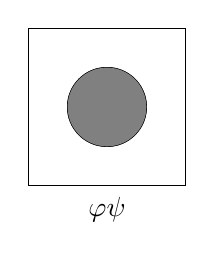
\begin{tikzpicture}
    \def\vennA{(-0.0,-0.0) circle (0.5)}
    \def\vennB{(0.0,0.0) circle (0.5)}

    \draw \vennB node [below] {};
    \draw \vennA node [above] {};
    \begin{scope}
      \fill[gray] \vennA;
    \end{scope}
    
    \frameVenn
    \draw (0, -1.3) node {$\varphi \equivalent \psi$};
  \end{tikzpicture}
}

\newcommand\forwardVenn{
  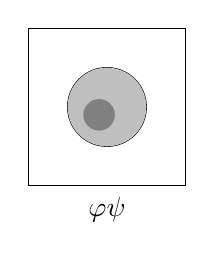
\begin{tikzpicture}
    \def\vennA{(-0.1,-0.1) circle (0.2)}
    \def\vennB{(-0.0,-0.0) circle (0.5)}

    \draw \vennB node [below] {};
    \draw \vennA node [above] {};
    \begin{scope}
      \fill[lightgray] \vennB;
    \end{scope}
    \begin{scope}
      \fill[gray] \vennA;
    \end{scope}
    
    \frameVenn
    \draw (0, -1.3) node {$\varphi \forward \psi$};
  \end{tikzpicture}
}

\newcommand\reverseVenn{
  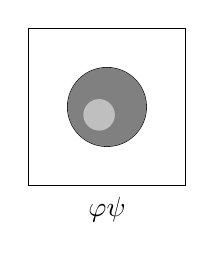
\begin{tikzpicture}
    \def\vennA{(-0.1,-0.1) circle (0.2)}
    \def\vennB{(0.0,0.0) circle (0.5)}
    
    \draw \vennB node [below] {};
    \draw \vennA node [above] {};
    \begin{scope}
      \fill[gray] \vennB;
    \end{scope}
    \begin{scope}
      \fill[lightgray] \vennA;
    \end{scope}
    
    \frameVenn
    \draw (0, -1.3) node {$\varphi \reverse \psi$};
  \end{tikzpicture}
}

\newcommand\negateVenn{
  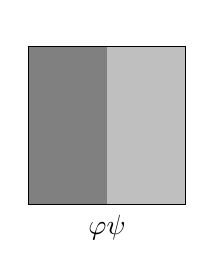
\begin{tikzpicture}
    \def\vennA{(0,-1) rectangle (1,1)}
    \def\vennB{(-1,-1) rectangle (0,1)}
    
    \draw \vennB node [below] {};
    \draw \vennA node [above] {};
    \begin{scope}
      \fill[gray] \vennB;
    \end{scope}
    \begin{scope}
      \fill[lightgray] \vennA;
    \end{scope}
    
    \frameVenn
    \draw (0, -1.3) node {$\varphi \negate \psi$};
  \end{tikzpicture}
}

\newcommand\alternateVenn{
  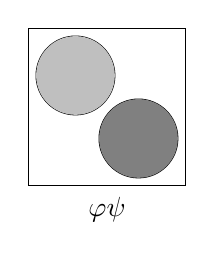
\begin{tikzpicture}
    \def\vennA{(-0.4,0.4) circle (0.5)}
    \def\vennB{(0.4,-0.4) circle (0.5)}
    
    \draw \vennB node [below] {};
    \draw \vennA node [above] {};
    \begin{scope}
      \fill[gray] \vennB;
    \end{scope}
    \begin{scope}
      \fill[lightgray] \vennA;
    \end{scope}
    
    \frameVenn
    \draw (0, -1.3) node {$\varphi \alternate \psi$};
  \end{tikzpicture}
}

\newcommand\coverVenn{
  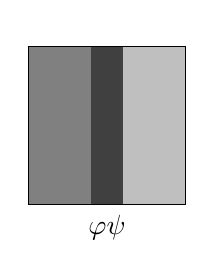
\begin{tikzpicture}
    \def\vennA{(-0.2,-1) rectangle (1,1)}
    \def\vennB{(-1,-1) rectangle (0.2,1)}
    
    \draw \vennB node [below] {};
    \draw \vennA node [above] {};
    \begin{scope}
      \fill[gray] \vennB;
    \end{scope}
    \begin{scope}
      \fill[lightgray] \vennA;
    \end{scope}
    \begin{scope}
      \clip \vennA;
      \fill[darkgray] \vennB;
    \end{scope}
    
    \frameVenn
    \draw (0, -1.3) node {$\varphi \cover \psi$};
  \end{tikzpicture}
}

%
% -----
% A playground for testing out figures
% -----
%
\newcommand\playground{
\begin{tikzpicture}[grow cyclic]
\tikzstyle{level 1}=[level distance=8mm,sibling angle=60]
\tikzstyle{level 2}=[level distance=4mm,sibling angle=45]
\tikzstyle{level 3}=[level distance=2mm,sibling angle=30]
\coordinate [rotate=-90] % going down
child foreach \x in {1,2,3}
{child foreach \x in {1,2,3}
{child foreach \x in {1,2,3}}};
\end{tikzpicture}

}
